% !TEX program = pdflatex
% !BIB program = bibtex
%
% Ecology Letters submission format (Letter article type).
% Reformatted from the original PNAS sources; all PNAS class files removed.
% Standard article class, double spacing, continuous line numbers, author-year (natbib) citations.

\documentclass[12pt]{article}

\usepackage[T1]{fontenc}
\usepackage[utf8]{inputenc}
\usepackage{mathpazo}
%\usepackage{lmodern}
\usepackage[a4paper,margin=1in]{geometry}
\usepackage{setspace}
\usepackage{lineno}
\usepackage{graphicx}
\usepackage{xcolor}
\usepackage{amsmath,amssymb}
\usepackage{booktabs}
\usepackage{enumitem}
\usepackage{float}
\usepackage[round,semicolon,authoryear]{natbib}
\usepackage{url}
\usepackage[hidelinks]{hyperref}

% Custom math macros carried over from the original sources.
\newcommand{\R}{\mathbb{R}}
\newcommand{\E}{\mathbb{E}}
\newcommand{\Z}{\mathbb{Z}}
\newcommand{\I}{\mathbb{I}}

\graphicspath{{figs/}}

\doublespacing
\linenumbers

\begin{document}

% ================= Title page =================
\thispagestyle{empty}
\begin{flushleft}

{\Large\bfseries Mixotrophic interactions drive a complex marine food web to the edge of instability}

\vspace{1.5em}
\textbf{Running title:} Mixotrophy drives plankton to instability

\vspace{1.5em}
Pablo Almaraz\textsuperscript{1,*}, Suzana G. Leles\textsuperscript{2,3}, David Garc\'{i}a-Callejas\textsuperscript{4,5} and Oscar Godoy\textsuperscript{6}

\vspace{1em}
\textsuperscript{1}Department of Ecology and Coastal Management, Instituto de Ciencias Marinas de Andaluc\'{i}a, CSIC, Puerto Real, 11519, Spain \\
\textsuperscript{2}Department of Marine and Environmental Biology, University of Southern California, Los Angeles, CA, USA \\
\textsuperscript{3}Department of Marine Science, University of Texas at Austin, Austin, TX, USA \\
\textsuperscript{4}School of Biological Sciences, University of Canterbury, Private Bag 4800, Christchurch 8140, New Zealand \\
\textsuperscript{5}Unitat d'Ecologia, Departament de Biologia Animal, Biologia Vegetal i Ecologia, Universitat Aut\`{o}noma de Barcelona, Cerdanyola del Vall\`{e}s, 08193, Spain \\
\textsuperscript{6}Estaci\'{o}n Biol\'{o}gica de Do\~{n}ana (EBD-CSIC), Am\'{e}rico Vespucio 26, Sevilla, 41092, Spain

\vspace{1em}
ORCID: \\
Pablo Almaraz \href{https://orcid.org/0000-0003-1416-2695}{0000-0003-1416-2695} \\
Suzana G. Leles \href{https://orcid.org/0000-0002-7819-5851}{0000-0002-7819-5851} \\
David Garc\'{i}a-Callejas \href{https://orcid.org/0000-0001-6982-476X}{0000-0001-6982-476X} \\
Oscar Godoy \href{https://orcid.org/0000-0003-4988-6626}{0000-0003-4988-6626}

\vspace{1em}
\textsuperscript{*}Correspondence: Pablo Almaraz, E-mail: \href{mailto:pablo.almaraz@csic.es}{pablo.almaraz@csic.es}

\vspace{1.5em}
\textbf{Statement of authorship (CRediT):} \textbf{Pablo Almaraz:} conceptualization, methodology, software, formal analysis, writing -- original draft, writing -- review \& editing. \textbf{Suzana G. Leles:} conceptualization, data curation, resources, writing -- original draft, writing -- review \& editing. \textbf{David Garc\'{i}a-Callejas:} conceptualization, writing -- review \& editing. \textbf{Oscar Godoy:} conceptualization, methodology, writing -- review \& editing.

\vspace{1em}
\textbf{Data accessibility statement:} Should the manuscript be accepted, the data and code supporting the results will be archived in a public repository (GitHub and Zenodo) and the data DOI will be included at the end of the article.

\vspace{1em}
\textbf{Competing interests:} The authors declare no competing interests.

\vspace{1em}
\textbf{Article type:} Letter

\vspace{1em}
\textbf{Manuscript information:} abstract, 141 words; main text, $\sim$4{,}770 words; 81 references; 6 figures; 0 tables; 0 text boxes.

\vspace{1em}
\textbf{Keywords:} network theory; Bayesian inverse model; coexistence; mixotrophy; stochastic structural stability.

\end{flushleft}

\clearpage

% ================= Abstract =================
\begin{center}\textbf{\large Abstract}\end{center}

\noindent Food web theory typically casts biotic interactions as competition or predation between primary producers and consumers, ignoring mixotrophs: protists that combine photosynthesis and phagotrophy. We investigate how mixotrophy shapes long-term coexistence and food web stability using a ten-year time series of weekly biomass for ten plankton functional groups, fitted with a Bayesian non-linear Lotka-Volterra model that accounts for environmental variability and interspecific interactions. We detect a small-world module of positive and negative interactions between heterotrophs and non-constitutive mixotrophs of nano- and micro-plankton size classes. Contrary to expectations, mixotrophy does not promote structural stability; rather, it pushes the community to the edge of instability, inducing highly reactive dynamics. This behavior disappears when mixotrophy is ignored by grouping taxa under the traditional autotroph versus heterotroph dichotomy. Accounting for mixotrophy is therefore essential to predict the persistence of marine communities in an ever-changing world.

\clearpage

% ================= Main text =================
\section*{Introduction}

Ecologists have long sought to understand the role of biotic interactions in modulating multiple key features of ecological communities. Prior work has shown that the sign, strength, and architecture in which interactions are embedded modulate the maintenance of biodiversity \citep{Levine2009,Bascompte2006a,McCann2010,gellner2023}, the stability and resilience of ecological communities to external perturbations \citep{Mougi2012,Kondoh2015}, as well as their functioning \citep{Cardinale2011,Godoy2020}. Yet, the vast majority of studies have reached these conclusions by assuming organisms interact in particular, fixed ways. For instance, plants compete for resources, pollinators establish mutualistic relationships with plants, and species interact antagonistically in food webs based on their feeding preferences. This classic vision collides with cumulative evidence showing the diffuse behavior of species within communities. As counterexamples, plants can also facilitate one another by ameliorating adverse abiotic conditions \citep{brooker2008}, pollinators can also harm flowers and reduce plant fitness \citep{magrach2017}, and commensalism and amensalism are common features in food webs \citep{sanders2012}. Conceptually, the continuous nature of biotic interactions would be better reflected without assuming sharply defined boundaries in their effects \citep{Holland2009, Gomez2023, buche2025}. However, how to rigorously implement this diffuse perspective and its consequences for understanding ecosystem dynamics remains unclear.

A globally relevant system that presents diffuse boundaries of biotic interactions is represented by the microscopic organisms that inhabit the sunlit ocean. Plankton communities are highly diverse in terms of phylogeny, size, and function, displaying versatile metabolic strategies \citep{Worden2015}. Although plankton communities have been traditionally studied under the paradigm of a plant-animal dichotomy (Fig.~\ref{fig:conceptual_web}A), most protist taxa (except diatoms) can act as both consumers and producers through mixotrophy (Fig.~\ref{fig:conceptual_web}B; \citep{Stoecker2016,selosse2017}). Mixotrophic protists combine photosynthesis with prey ingestion to achieve metabolic flexibility \citep{Flynn2013,lambert2022}. They are ubiquitous in the global ocean \citep{leles2017oceanic, faure2019mixotrophic,Edwards2019} and may account for most bacterial consumption in oligotrophic seas \citep{hartmann2012mixotrophic}. Global ocean models show that the presence of mixotrophy increases trophic transfer and the export of carbon from surface waters \citep{Ward2016}. A basic distinction can be made between mixotrophs that possess (constitutive) or acquire (non-constitutive) the ability to photosynthesize \citep{Mitra2016}. While both occur in a continuum of metabolic strategies \citep{Stoecker2016,wilken2020contrasting}, non-constitutive mixotrophs must steal the plastids from their phototrophic prey or host phototrophic endosymbionts to fix inorganic carbon \citep{Stoecker2016,johnson2023functional}. These diverse strategies suggest that mixotrophs can have contrasting effects on the stability of plankton communities. For example, due to the need to periodically acquire new plastids, acquired phototrophy was found to promote coexistence between a mixotroph and its prey, but the degree to which they rely on carbon obtained through photosynthesis can shift systems from a coexistence equilibrium to cyclic (bloom) dynamics \citep{Moeller2016}. However, the combined effects of environmental variation, self-limiting processes, and interspecific interactions on promoting the long-term persistence of mixotrophy within highly diverse plankton communities remain poorly understood.

\begin{figure}[t!]
	\centering
	\includegraphics[width=\linewidth]{figs/Fig1_study_area_timeseries.pdf}
	\caption{Study area and plankton community time series at station L4 (Western Channel Observatory, 50.25\,N, 4.22\,W). \textbf{(A)} April climatology of surface chlorophyll-a concentration (2007--2014) from the Copernicus Marine multi-sensor L4 reprocessed ocean-color product (OCEANCOLOUR\_ATL\_BGC\_L4\_MY\_009\_118; ingests Sentinel-3 OLCI together with the heritage sensors MERIS, MODIS-Aqua, VIIRS and SeaWiFS over the 2007--2014 climatology window). The inset locates the Western English Channel within the European Atlantic shelf. \textbf{(B)} Concurrent environmental drivers measured at the same station: surface temperature, modeled mixed-layer depth, in-water chlorophyll-a concentration, and four inorganic nutrient pools (nitrate, ammonium, silicate, phosphate). \textbf{(C--E)} Biomass time series (log-scaled, $\mu$g C L$^{-1}$) of the ten plankton functional types, grouped by trophic strategy: \textbf{(C)} autotrophs, \textbf{(D)} constitutive (NanoCMs, MicroCMs) and non-constitutive (GNCMs, SNCMs) mixotrophs, \textbf{(E)} strict heterotrophs. Each line is color-coded by functional type.}
	\label{fig:study_area_ts}
\end{figure}

\begin{figure}[t!]
	\centering	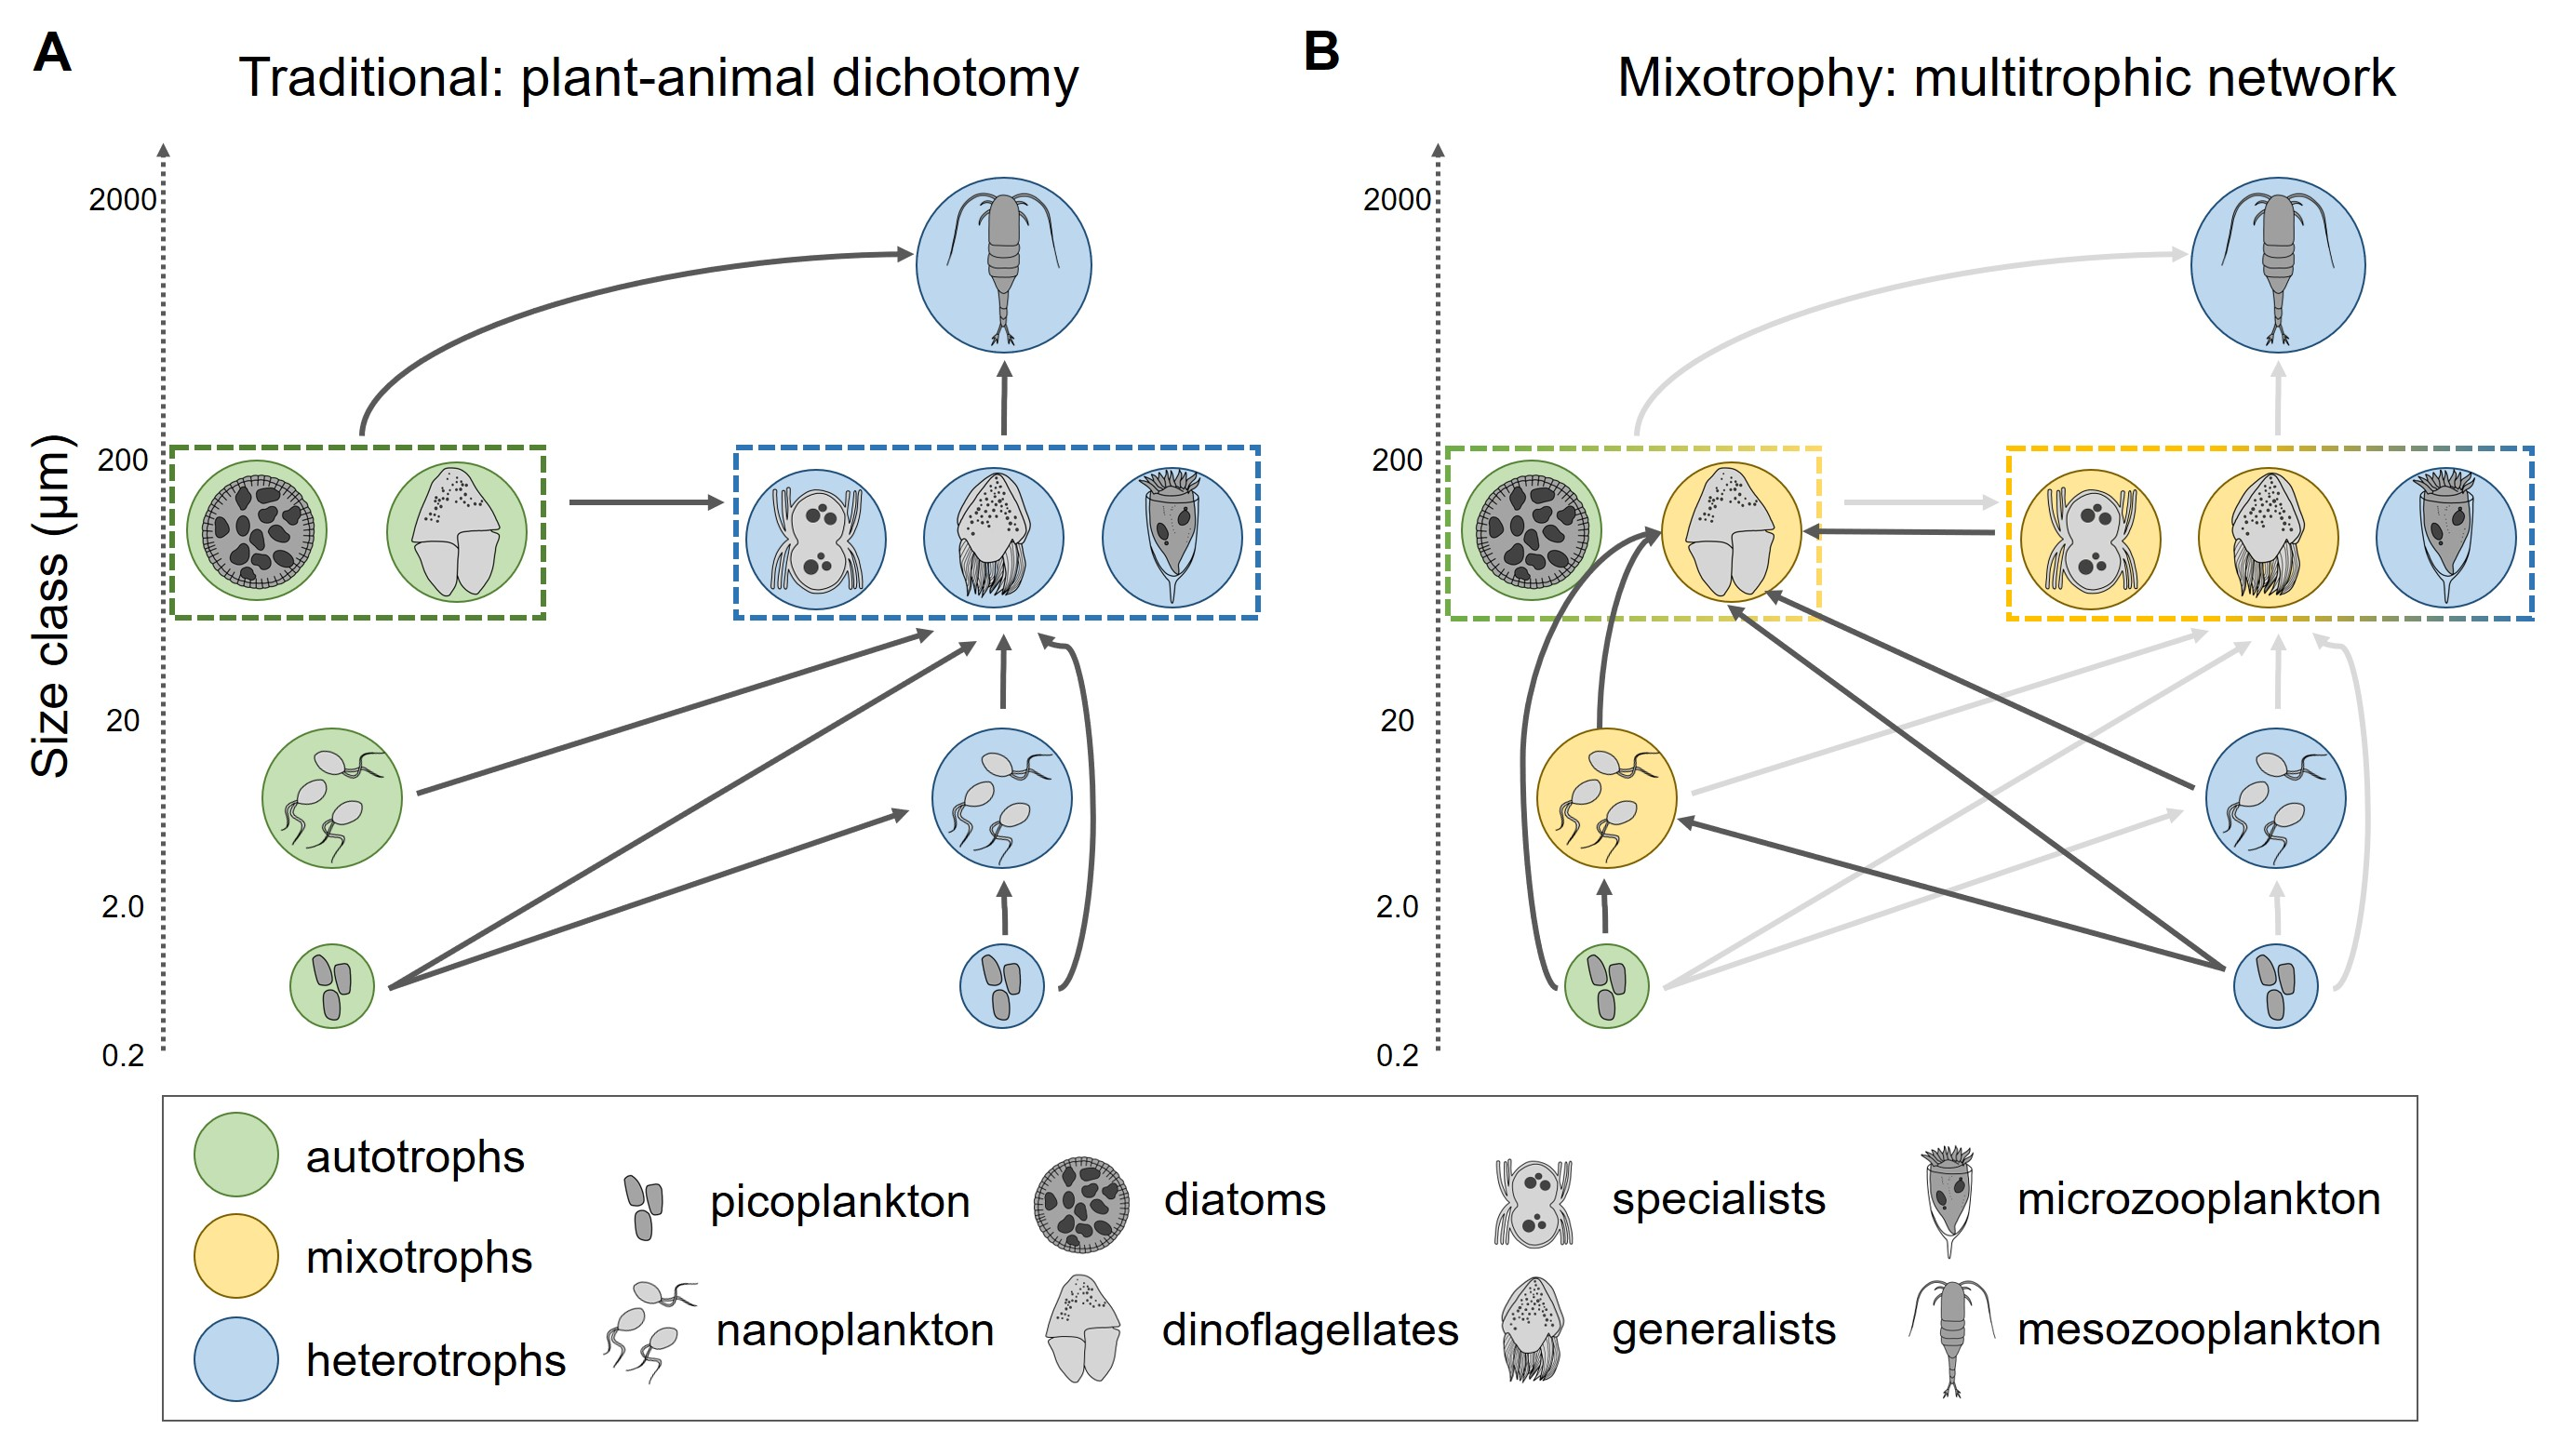
\includegraphics[width=\linewidth]{figs/foodwebs.jpg}
	\caption{Conceptual representation of plankton food webs. The traditional approach to describe plankton communities splits functional types according to size and between autotrophs and heterotrophs, following the plant-animal dichotomy (A). In reality, many functional types are mixotrophs combining photosynthesis with the ingestion of prey (B). For example, many taxa within nanophytoplankton and dinoflagellates are constitutive mixotrophs. Many non-constitutive mixotrophs are commonly considered part of the microzooplankton; here, we separate non-constitutive mixotrophs into specialists (taxa that rely on specific prey to acquire plastids) and generalists (taxa that rely on diverse prey to acquire plastids). Arrows describe potential predator-prey interactions and are common to two or more functional types when these are included within dashed rectangles. The arrows described in panel A were shaded in panel B to highlight the new interactions when mixotrophy is included in the food web. Plankton drawings illustrate one representative of the different functional types.}
	\label{fig:conceptual_web}
\end{figure}

To address this gap of knowledge, and more generally, to build solid bridges connecting the structure of biotic interactions with the long-term dynamics of ecological communities, we must address three limitations. First, we need to account for the fact that plankton communities are subjected to continuous variation in environmental conditions, and population trajectories are highly influenced by dispersal processes and stochastic events \citep{Thompson2020,Shoemaker2019}. Second, we need to validate whether the structure of biotic interactions describes the long-term population dynamics of the system. This lack of validation is widespread in empirical and experimental studies and commonly leads to misunderstandings in the long-studied relationship between community complexity and stability. While the seminal work by \citet{May1972} posits that the higher the number of interactions and species in a system, the more unstable a community is expected to be, this pattern is reversed if we focus on the subset of feasible communities. In this case, the more stable communities turn out to be the more complex ones \citep{Roberts1974}. Third, the same modeled structure of biotic interactions can produce quite contrasted long-term dynamics due to historical and contingency factors such as species abundances, legacy effects, or variation in intrinsic growth rates \citep{Song2020a}. Therefore, we need to correctly characterize the uncertainty associated with the estimated interaction structures and the emergent system dynamics.

Here, we assess the structure of biotic interactions that mixotrophic protists display in the ocean. We implemented an inverse Bayesian modeling approach and applied it to a long-term time series (10-yr) of weekly plankton biomass fluctuations of ten different functional groups of autotrophs, mixotrophs, and heterotrophs spanning over four orders of magnitude in body size (Fig.~\ref{fig:conceptual_web}B). Our approach simultaneously accounts for the effects of environmental drivers as well as sampling frequency and environmental stochasticity. With this information at hand, we then investigate the role of mixotrophy in shaping the structure of plankton interactions. We explore whether mixotrophs are involved in a complex set of interspecific interactions within the whole plankton food web, or in contrast, their temporal dynamics are mostly driven by self-limiting processes. Finally, because we found that mixotrophs are tightly linked to other plankton functional groups, we investigate the role of the assessed interaction structure in promoting the stability and feasibility (i.e., long-term persistence) of the whole plankton community. These stability analyses, acknowledging the mixotroph components of the food web, were critically compared to those obtained with a traditional food web classification that assumes the plant-animal dichotomy (Fig.~\ref{fig:conceptual_web}A). We discuss the importance of adopting a diffuse perspective to investigate complex systems, such as marine plankton communities, to better understand how biodiversity is maintained in ecosystems governed by organisms able to vary the sign and strength of their biotic interactions.

\section*{Material and methods}

\subsection*{The L4 dataset}

We analyzed a long-term time series dataset obtained at the L4 monitoring station, located in the Western English Channel, UK (50°15N, 4°13W). This time series is part of the Western Channel Observatory (\url{http://www.westernchannelobservatory.org.uk/}). The L4 station (RV Plymouth Quest) is a coastal temperate site and comprises one of the longest plankton time series worldwide. The abiotic variables affecting plankton growth and which are included in our analysis were temperature, salinity, mixed layer depth, inorganic nutrients, chlorophyll-a, and carbon biomass of all plankton functional types \citep{Smyth2010,Widdicombe2010,Atkinson2015,Tarran2015}. Both plankton carbon biomass and environmental data analyzed spanned over a period of 10 years, from 2006 to 2015 with an approximately one-week resolution. We did not use data collected before 2006 due to a lack of taxonomic resolution that hampered the identification of mixotrophic taxa. The major nutrients, nitrate + nitrite, silicate, and phosphate, follow a similar seasonal pattern as temperature, whereas Chlorophyll-a levels are consistently low during late autumn and winter, and higher during spring and summer.

\subsection*{Functional grouping}

We implemented a two-step process to classify the wide diversity of trophic strategies and cell sizes of the L4 plankton dataset (Fig.~\ref{fig:conceptual_web}). Following previous studies, \citet{leles2021differences}, we first grouped taxa according to three main trophic strategies: autotrophs (producers), heterotrophs (consumers), or mixotrophs (producers and consumers). We then further divided these three functional groups based on their mixotrophic functional diversity and size (ranging over four orders of magnitude, from pico- to meso- plankton, i.e., 0.2 $\mu$m -- 2 mm). In total, we obtained 10 functional groups: two autotrophs (picophytoplankton and diatoms), four heterotrophs (bacteria, nano-, micro-, and meso- zooplankton), and four mixotrophs (including constitutive and non-constitutive types) (Table S1). Briefly, mixotrophic taxa were divided following \citet{leles2021differences} as follows: constitutive mixotrophs included all autotrophic flagellates that possess their own photosystems. These were then divided into two mixotrophic types according to cell size, i.e., nano- (2--20 $\mu$m) and micro- (20--200 $\mu$m) plankton. Non-constitutive mixotrophs included all dinoflagellate and ciliate taxa known to acquire photosynthetic capacity from their autotrophic prey. These were then divided between specialist (mostly \textit{Mesodinium}) and generalist (mostly \textit{Strombidium}) mixotrophs according to their ability to obtain plastids from specific or diverse prey types, respectively. All non-constitutive forms were in the microplankton size class. Fig.~S2 in the SI Appendix shows time-series plots of each of the ten functional types considered.

\subsection*{Time series modeling of plankton community dynamics}

Because observing biotic interactions in open-ocean plankton communities is unfeasible for logistical and technical reasons, we inferred these interactions from temporal changes in biomass. To do this, we adopted a Bayesian inverse modeling approach through state-space methods (e.g., \citealp{Mutshinda2011,Almaraz2024}) to fit a Lotka-Volterra model with Ricker-type interactions. We chose a Ricker-type model because it allows us to parameterize positive and negative interactions \citep{mayfield2017}. The model also includes the environmental abiotic effects on the intrinsic growth of the L4 time-series community plankton biomass. Briefly, a state-space scheme is a fully stochastic model in which uncertainty is segregated into two equations. First, a state equation, which models the system under study with an associated process variance. Second, an observation equation, linked to the state equation through a measurement process with observation error \citep{Clark2004,Mutshinda2011,Almaraz2024}. In this approach, the `true' state of the system (i.e., plankton biomass in our study) is thus regarded as unobserved, or latent \citep{Durbin2001}. Therefore, uncertainty is optimally handled and propagated across the model structure, therefore reducing the bias in the estimation of both the interaction network and the environmental abiotic effects on plankton growth (see \citep{Mutshinda2009,Mutshinda2011,Almaraz2024}).

\subsubsection*{Structure of the inverse state-space model}

The state (process) equation of the discrete-time Lotka-Volterra-Ricker model, written on the log-biomass scale, is
\begin{equation}\label{LVRickerDiscr}
	\begin{split}
		n_{i,t+\delta_{t}} \;=\; n_{i,t} + \delta_{t}\, r_{i}\!\left[\,1 - \frac{N_{i,t}}{K_{i}} + \frac{1}{K_{i}}\sum_{j\neq i}^{s}\alpha_{ij}\,N_{j,t}\right] \\
		\quad+\, \delta_{t}\sum_{m=1}^{p}\beta_{i,m}\,c_{m,t} \,+\, \delta_{t}\,\epsilon_{i,t}, \\
		\text{for}\;\; i=1,\ldots,s.
	\end{split}
\end{equation}
Here $n_{i,t}=\log_{e}N_{i,t}$ is the latent (unobserved) log-biomass of functional type $i$ at time $t$, and $N_{j,t}$ is the corresponding raw latent biomass of functional type $j$. The variable $\delta_{t}$ is the sampling interval between successive events; although most lapses among samplings were of one week, this figure varied across the full sampling scheme (for instance, there are no data available for some months). Rather than interpolating or imputing data, we treat this scheme as a case of uneven sampling \citep{Clark2004,Clark2007}, which affects the estimation of parameters and process error in Eqn.~\ref{LVRickerDiscr}. The $r_{i}$ are the per-capita intrinsic (instantaneous) rates of increase for each functional type, and the $K_{i}$ are their carrying capacities. The coefficients $\alpha_{ij}$ measure the per-capita direct effect of type $j$ on the population growth rate of type $i$, relative to the impact of type $i$ on itself, with all other species held constant \citep{Levins1968,Novak2016}; the sign of $\alpha_{ij}$ encodes the type of interaction (positive: facilitation; negative: competition or predation). Intra-specific self-limitation is carried by the dedicated term $-N_{i,t}/K_{i}$, so the alpha matrix $\mathbf{A}=(\alpha_{ij})$ has zero diagonal entries, $\alpha_{ii}=0$; the inner sum in Eqn.~\ref{LVRickerDiscr} therefore runs over $j\neq i$. The matrix $\boldsymbol{\beta}\in\R^{s\times p}$, with entries $\beta_{i,m}$, holds the impacts of the $p$ environmental covariates $c_{m,t}$ on the growth rate of each type. The vector $\boldsymbol{\epsilon}_{t}=(\epsilon_{1,t},\ldots,\epsilon_{s,t})^{T}$ collects the environmental-stochasticity terms, with $\boldsymbol{\epsilon}_{t}\sim\mathcal{MVN}(\mathbf{0},\Sigma)$; the diagonal entries $\sigma_{i}^{2}$ of $\Sigma$ measure the variance of unmodeled environmental drivers acting on each type, and the off-diagonal entries $\mathrm{cov}(\epsilon_{i},\epsilon_{j})$ measure shared latent forcing.

The state equation in Eqn.~\ref{LVRickerDiscr} is linked to the biomass samples through an observation model,
\begin{equation}\label{LVR_Obs_model}
	y_{i,t} \;=\; n_{i,t} + \rho_{i,t}, \qquad \rho_{i,t} \sim \mathcal{N}(0,\tau_{i}^{2}),
\end{equation}
with measurement-error variances $\tau_{i}^{2}$ that we assume uncorrelated across functional types. The initial state of each latent log-biomass is $n_{i,0}\sim\mathcal{N}(\mu_{i,0},\sigma_{0,i}^{2})$, with prior mean $\mu_{i,0}$ and variance $\sigma_{0,i}^{2}$ specific to each type. The explicit Bayesian specification, prior choices, and posterior derivation are given in the SI Appendix.

\subsection*{Community coexistence and stability}

The deterministic skeleton of the state equation in Eqn.~\ref{LVRickerDiscr} converges to an equilibrium $\mathbf{N}^{*}$ when $\mathbf{N}_{t+1}=\mathbf{N}_{t}$. Setting the increment in Eqn.~\ref{LVRickerDiscr} to zero, multiplying the $i$-th row by $K_{i}>0$, and using $\alpha_{ii}=0$ to extend the inner sum over all $j$ yields, in matrix form,
\begin{equation}\label{eqn:equilibrium_main}
	(\mathbf{I}-\mathbf{A})\,\mathbf{N}^{*} \;=\; \mathbf{K}, \qquad \mathbf{N}^{*} \;=\; (\mathbf{I}-\mathbf{A})^{-1}\,\mathbf{K},
\end{equation}
where the closed form holds whenever $\mathbf{I}-\mathbf{A}$ is invertible (a sufficient condition is the spectral radius $\rho(\mathbf{A})<1$). The equilibrium is \textit{feasible} when every component of $\mathbf{N}^{*}$ is strictly positive, meaning that every functional type maintains a viable population \citep{Roberts1974}. Because the interaction matrix $\mathbf{A}$ and the carrying capacities $\mathbf{K}$ are estimated as posterior distributions, the \textit{probability of feasibility} is defined as the fraction of posterior draws for which $\min_{i}N_{i}^{*}>0$. This provides a probabilistic measure of community coexistence under parameter uncertainty \citep{Almaraz2024}.

If a feasible equilibrium exists, the \textit{dynamical stability} of the fitted process is assessed by linearizing Eqn.~\ref{LVRickerDiscr} about $\mathbf{n}^{*}=\log\mathbf{N}^{*}$. Because the state-space model is written on the log-biomass scale, the relevant Jacobian is $\mathbf{J}=\partial\boldsymbol{\Phi}/\partial\mathbf{n}^{T}\bigl|_{\mathbf{n}^{*}}$, whose entries are derived in the SI Appendix:
\begin{equation}\label{eqn:jacobian_entries_main}
	J_{ii} \;=\; 1 - \delta_{t}\,\frac{r_{i}\,N_{i}^{*}}{K_{i}}, \qquad J_{ij}\bigl|_{j\neq i} \;=\; +\,\delta_{t}\,\frac{r_{i}\,\alpha_{ij}\,N_{j}^{*}}{K_{i}}.
\end{equation}
In compact form, $\mathbf{J}=\mathbf{I}-\delta_{t}\,\mathbf{R}\,\mathbf{K}_{\mathrm{d}}^{-1}\,(\mathbf{I}-\mathbf{A})\,\mathbf{N}^{*}_{\mathrm{d}}$, with $\mathbf{R}=\mathrm{diag}(\mathbf{r})$, $\mathbf{K}_{\mathrm{d}}=\mathrm{diag}(\mathbf{K})$ and $\mathbf{N}^{*}_{\mathrm{d}}=\mathrm{diag}(\mathbf{N}^{*})$ (see SI Appendix). For discrete-time systems, the equilibrium is stable when the spectral radius of $\mathbf{J}$ is strictly less than 1, that is, when every eigenvalue of $\mathbf{J}$ lies inside the unit disc in the complex plane \citep{Elaydi2005}. We define the \textit{probability of dynamical stability} as the fraction of posterior draws of $\mathbf{J}$ satisfying this criterion. From the eigenvalue spectrum of $\mathbf{J}$, we derive three complementary scalar metrics that capture different aspects of the system's response to perturbations:

\begin{itemize}[nosep]
	\item \textbf{Resilience} ($\mathrm{R}_{\infty}$): the inverse of the modulus of the dominant eigenvalue of $\mathbf{J}$, $\mathrm{R}_{\infty}=1/\max_{\lambda}|\lambda(\mathbf{J})|$, in units of $t^{-1}$; it measures the asymptotic rate of return to equilibrium after a small perturbation of initial conditions \citep{Ives2003,Arnoldi2016a}. Higher values indicate faster recovery.
	\item \textbf{Reactivity} ($\mathrm{R}_{0}$): the maximum instantaneous amplification of a perturbation about the equilibrium, $\mathrm{R}_{0}=\ln\!\sqrt{\lambda_{\max}(\mathbf{J}^{T}\mathbf{J})}$ \citep{Snyder2010a}. Positive reactivity means that the system initially amplifies disturbances even when it is asymptotically stable, a transient excursion that can trigger large biomass fluctuations.
	\item \textbf{Stochastic structural stability} ($\mathcal{I}_{s}$): the minimal intensity of continuous white-noise perturbation that destabilizes the linearized system, $\mathcal{I}_{s}=-\delta_{t}^{-1}\ln\!\bigl(1-1/\lVert(\mathbf{I}-\mathcal{J})^{-1}\rVert\bigr)$ with $\mathcal{J}=\mathbf{J}\otimes\mathbf{J}$ \citep{Arnoldi2016b}. This metric jointly captures the response to perturbations of state variables and the response to sustained stochastic forcing of the parameters; large values of $\mathcal{I}_{s}$ indicate a community robust to both external shocks and internal variability.
	\item \textbf{Probability of feasibility}: the fraction of posterior equilibrium vectors $\mathbf{N}^{*}$ in which every functional type attains a strictly positive abundance \citep{Almaraz2024}. While the previous metrics characterize how the system responds to perturbations near the equilibrium, feasibility quantifies whether the equilibrium itself sustains all functional types simultaneously; a decline in this probability across alternative community configurations signals a contraction of the feasibility domain and increased vulnerability to species loss \citep{Almaraz2024}.
\end{itemize}

Together, these four metrics provide a comprehensive picture of community stability: resilience captures the long-term return rate, reactivity reveals the short-term vulnerability to transient amplification, stochastic structural stability quantifies the overall robustness of coexistence to sustained perturbations, and the probability of feasibility assesses whether the equilibrium itself is viable. All metrics are computed from the full posterior distribution, propagating the uncertainty inherent in the estimated interactions and growth parameters. The mathematical derivations are provided in the SI Appendix.

\section*{Results}

\subsection*{Estimation of inter-type interactions and environmental effects}

\begin{figure}[t!]
	\centering	\includegraphics[width=0.5\linewidth]{figs/Main_timeseries.pdf}
	\caption{Posterior Predictive Checks performed with the stochastic formulation of the Lotka-Volterra-Ricker model shown in Eqn. \ref{LVRickerDiscr} fitted to the community time series of the plankton community. The core small-world of 5 interacting functional types is shown. Blue dots \textcolor{blue}{$\bullet$} denote the weekly measured biomass for each functional type, and red lines \textcolor{red}{{\Huge -}} denote the posterior predicted average of 3000 synthetic biomass time series for each functional type. Red shaded regions contain the 90\% HDI of the posterior predictions for each type.}
	\label{fig:timeseries}
\end{figure}

The simulated time-series derived from the fitted posterior distribution closely matched the observed dynamics (Fig. \ref{fig:timeseries}). These dynamics were driven by only a few significant interactions between functional groups. This means that the posterior interaction matrix $ \mathbf{A} $ was very sparse in spite of a weakly informative prior distribution for the probability of inclusion of interactions between functional groups (Fig.~\ref{fig:Interact_prob_alpha}). In particular, the posterior distribution of the probability of inclusion of interactions between functional groups in the community dynamics model had a maximum posterior mode of 0.036 [0.01, 0.090]. In summary, out of a potential number of 90 inter-type interactions, only 5 yielded a Bayes factor worth mentioning (Fig.~S3 in the SI Appendix).

\begin{figure}[t!]
	\centering
	\includegraphics[width=1\linewidth]{figs/Interaction_networks_wlegend.pdf}
	\caption[Network of posterior probability of interactions and interactions]{\footnotesize In \textbf{A}, network of posterior probability of interactions, constructed with the marginal probabilities of interactions across the ensemble of posterior networks explored by the SSVS algorithm. Green arrows (edges) indicate the direction of the effect and its magnitude (thickness), from 0 to 1. Note that in our modeling approach, self-limiting effects are fixed to 1 and thus are always selected, and interspecific interactions are scaled compared to intraspecific ones  (see Methods, section ``Structure of the inverse state-space model''). In \textbf{B}, network of inter-type interactions (i.e., interactions between functional groups) as expressed in the $\alpha$-matrix. These links measure the direct impact of the average species \textit{j} individual on species \textit{i}'s growth rate, relative to \textit{i}'s effect on its own growth rate (\citealp{Novak2016}). Interactions are depicted as directed arrows. Blue arrows denote a negative effect of the $\alpha_{ij}$, while red arrows denote a positive impact; arrow thickness depicts the relative magnitude of the effect. Note that the posterior values are given for the average of the posterior evaluated at the slab.}
	\label{fig:Interact_prob_alpha}
\end{figure}

This sparse structure of posterior probability of interactions involves the following functional groups with decisive support conditioned on the observed data: nanozooplankton, non-constitutive mixotrophs (both generalists, e.g., \textit{Strombidium} and specialists, e.g., \textit{Mesodinium}), microzooplankton, and mesozooplankton (Fig. \ref{fig:Interact_prob_alpha}A). These functional types shape a ``small-world'' of strong interactions across groups, with nanozooplankton being the keystone group. According to the interaction matrix (Fig. \ref{fig:Interact_prob_alpha}B), there is, on average, a positive impact of non-constitutive mixotrophs on the growth rate of nanozooplankton, while the impact of microzooplankton on nanozooplankton is strongly negative. Nanozooplankton had no direct impact on other functional types (i.e., no outgoing arrow was detected from this functional type).

The effects of nutrients and temperature on the growth rate of each functional type were generally negative, with all other variables having a mixed, generally weak, effect (Fig.~S4 in the SI Appendix). Only the dynamics of heterotrophic bacteria and generalist non-constitutive mixotrophs were largely independent of nutrients and temperature. Temperature and inorganic nutrients were strongly and negatively correlated, as expected based on oceanographic conditions (i.e., colder temperatures are usually associated with higher concentrations of inorganic nutrients). The cross-correlation of the biomass of functional types in the fluctuations of the common environment, as measured through the environmental stochastic effects (the matrix $\Sigma$ that governs the multivariate noise $\boldsymbol{\epsilon}_{t}$ in Eqn.~\ref{LVRickerDiscr}), is positive in nearly all cases (see Fig.~S5 in the SI Appendix).

\subsection*{Stability, feasibility and community coexistence}

A primary goal of ecologists is to investigate whether the inferred interactions allow an ecological community to persist in the long term -- that is, whether the system is both dynamically stable (i.e., able to absorb small perturbations) and feasible (i.e., all functional types maintain positive populations at equilibrium). By deriving the equilibrium of the population model, we observed that our plankton community is dynamically stable with a very large probability (effectively 100 \%, Fig. \ref{fig:Stability_Feasibility} a): all of the posterior estimated dominant eigenvalues of the Jacobian matrix fall within the unit circle. However, our analyses also suggest that the system is close to instability. Technically, this is observed because the posterior distribution of dominant eigenvalues is close to the nonhyperbolic case, where the dominant eigenvalue has modulus 1. We interpret such proximity to the edge of instability as indicating that the studied plankton system can propagate perturbations, although these are asymptotically absorbed in the long term.

To better capture the dynamical behavior of our system, several complementary analyses were performed. First, we found a relatively slow resilience (1.030 [1.006, 1.059] $ t^{-1} $, see Fig. \ref{fig:Stability_Feasibility}) indicating that population abundances change after perturbations. Second, we also found a strongly positively skewed distribution of reactivity (Fig.~\ref{fig:Stability_comparison}): although the maximum posterior mode was negative, the posterior distribution included a large mass of positive values (-0.030 [-0.126, 1.064]; 66 \% of the distribution included positive values). These positive reactivity values indicate a significant potential of the system to initially amplify perturbations before returning to its steady state. Finally, and in further agreement with these previous findings, we also found a relatively low stochastic structural stability (stochastic invariability) (0.003 [0.0002, 0.090]). This last result reinforces the idea that the plankton community is sensitive to perturbations in abundances or changes in the structure of biotic interactions. Despite being sensitive to perturbations, the marine community is a strongly feasible system with a posterior probability of feasibility at equilibrium for all functional types nearly 1 (Fig. \ref{fig:Stability_Feasibility}).

When these stability analyses were conducted through the classic lens of food web theory of plant-animal dichotomy, that is, autotrophs versus heterotrophs, we found that reactivity is clearly smaller without the presence of non-constitutive mixotrophs (Fig.~\ref{fig:Stability_comparison}). This result suggests that acquired phototrophy is responsible for propagating perturbations within the plankton community in the short-term. In the long-term, evaluations with and without non-constitutive mixotrophs indicate that the system is resilient, but mixotrophs reduce the amount of perturbations the system can handle before losing species (i.e., lower stochastic structural stability). These findings suggest that non-constitutive mixotrophs drive the plankton system to the edge of instability. Specifically, the probability of feasibility remained high across the three community configurations, but stochastic structural stability was markedly lower in the mixotrophic web, confirming that resolving mixotrophic interactions reveals a community closer to its stability boundary than traditional classifications would suggest (Fig.~\ref{fig:Stability_comparison}). From an ecological standpoint, the high reactivity of the mixotrophic web implies that even moderate environmental perturbations can trigger large transient fluctuations in community biomass before the system returns to equilibrium. Combined with the low stochastic structural stability, this indicates that the plankton community operates in a narrow range of combinations of population growth where small shifts in interaction strength or environmental forcing could push individual functional types below viable population sizes, with cascading consequences for trophic transfer and biogeochemical cycling \citep{Lotze2019}.

\begin{figure}[t!]
	\centering
	\includegraphics[width=\textwidth]{figs/Wrapped_stability.pdf}
	\caption[Posterior probability of stability and feasibility]{In (\textbf{a}), the posterior eigenvalues of the Jacobian matrix (see SI Appendix) are shown in the unit circle of the complex plane. The probability of stability is the fraction of eigenvalues with modulus strictly smaller than 1 in the posterior distribution. In (\textbf{b}), the posterior distribution of each component of the equilibrium vector $ \mathbf{N}^* $ is shown for each functional group; for comparison, the MAP estimate for the carrying capacities is shown as red circles. The probability of feasibility is the fraction of posterior estimates of the equilibrium vector that are strictly positive. NanoCMs: constitutive mixotrophs within the nanoplankton size class; MicroCMs: constitutive mixotrophs within the microplankton size class; GNCMs: generalist non-constitutive mixotrophs; SNCMs: specialist non-constitutive mixotrophs.}
	\label{fig:Stability_Feasibility}
\end{figure}

\section*{Discussion}

Our findings revealed that mixotrophs are key in the ensemble of a plankton food web in a coastal temperate sea. The small-world of interactions they create drives the system to the edge of instability in an otherwise feasible community (Figs. \ref{fig:Stability_Feasibility} and \ref{fig:Interact_prob_alpha}). These interspecific interactions emerge from the dual trophic role of non-constitutive mixotrophs: by combining acquired phototrophy with heterotrophy, they alleviate predation pressure on nanozooplankton while competing with microzooplankton for shared prey resources. In fact, when species were grouped according to the autotroph-heterotroph dichotomy (i.e., neglecting mixotroph functional grouping), we found that the interaction network was strongly rewired: the strong positive effects of non-constitutive mixotrophs on nanozooplankton disappeared, the community appeared governed by weaker, more diffuse interactions, and the system exhibited lower reactivity and higher stochastic structural stability (Fig.~\ref{fig:Stability_comparison}). This apparent stabilization is an artifact of lumping functionally distinct organisms, which masks the mechanistic interactions driving system dynamics. These key interactions between non-constitutive mixotrophs and heterotrophs are estimated with high confidence, suggesting that the ecological role of these groups and their net effect on other plankton taxa is conserved through time, despite variations in environmental or other abiotic conditions. Thus, in the plankton food web of the Western English Channel, mixotrophs can be considered as keystone taxa that contribute disproportionately to the dynamics and stability of the system.

Overall, we found that intraspecific interactions were stronger than interspecific interactions at equilibrium (Fig.~\ref{fig:Interact_prob_alpha}). This result was expected according to theory that predicts intraspecific interactions to be comparatively more important in highly connected and diverse communities \citep{Barabas2016}. Mixotrophy was the core of the interaction set of the analyzed plankton food web. The metabolic plasticity of mixotrophs can lead to asynchrony, which tends to stabilize biological systems. It is well recognized that species (or functional groups) can adapt and evolve to use different resources to decrease interspecific competition (e.g., \citealp{Moosmann2021}). This is clearly shown in our plankton food web, in which diverse trophic strategies and cell sizes result in weak interspecific interactions in the long-term. However, competition can also drive diversification within functional groups \citep{Svanback2007}. In fact, one can expect high trait diversity within a single plankton functional type \citep{Kruk2010,Kruk2011,Irwin2015}. This can in part explain why mixotrophic species fall within a continuum of nutritional modes from mainly phototrophic to mainly heterotrophic \citep{Stoecker2016}.

This diffuse nature of mixotrophic species may potentially promote important interspecific interactions depending on whether mixotrophs preferentially act as competitors or predators \citep{tittel2003mixotrophs}. The emergence of well-identified, comparatively strong interactions in a system otherwise regulated by self-limitation and environmental stochasticity may be detrimental to its stability, but there is little empirical support for this hypothesis \citep{McCann1998,Neutel2002}. We found evidence of this pattern in the Western English Channel plankton food web, where we uncovered a ``small world'' set of interactions between two types of non-constitutive mixotrophs and three of heterotrophs. Small world patterns are characterized by most functional groups being weakly connected except for a few that are highly linked \citep{Dunne2002,Sinha2005}. These can be widespread in diverse and complex food webs in nature, and they have been suggested to promote fast responses to perturbations \citep{Montoya2003}. Under the plant-animal dichotomy, the small-world pattern dissolves, and interactions become more evenly distributed among functional types, consistent with theoretical predictions that aggregating functionally diverse taxa artificially weakens apparent interspecific effects \citep{Barabas2016}.

The ``small world'' observed in this study involved heterotrophs and non-constitutive mixotrophs of nano- and microplankton size classes. These groups correspond to the main consumers of primary production in the oceans \citep{Schmoker2013}. By being smaller and having growth rates similar to their prey, nano- and micro-grazers can take advantage of an often-limited environment and respond quickly to increases in primary production \citep{Schmoker2013}. These mixotrophs are commonly classified as purely heterotrophic and grouped together with microzooplankton within ocean plankton models \citep{butenschon2016ersem, Ward2016} and ecological analyses \citep{segura2017community}. However, here we find that non-constitutive mixotrophs have a positive impact on nanozooplankton, contrary to microzooplankton (Fig.~\ref{fig:Interact_prob_alpha}). Despite having the same size range as microzooplankton, non-constitutive mixotrophs also acquire carbon from photosynthesis by stealing the plastids from their phototrophic prey \citep{johnson2023functional}. This relationship is obligate, and mixotrophs do not survive without functional acquired plastids \citep{McManus2012}. There are thus two reasons that could explain their positive impact on nanozooplankton: i) they ingest preferentially phototrophic prey to replace their plastids frequently \citep{Dolan2000} and ii) they acquire carbon and energy through photosynthesis \citep{johnson2023functional}; both mechanisms could alleviate the predation pressure on nanozooplankton. On the other hand, microzooplankton prey on nanozooplankton and also compete with them for pico-sized prey (e.g., bacteria) (Fig.~\ref{fig:conceptual_web}). This finding highlights the importance of disentangling the ecological roles of mixotrophs from their strict heterotrophic competitors. It is worth noting that non-constitutive mixotrophs typically exhibit lower biomass relative to their strict heterotrophic competitors in the Western English Channel. Despite this, the decisive Bayes factor support for NCM interactions (Fig.~S3 in the SI Appendix) indicates that our inverse modeling approach is sensitive enough to detect these effects, consistent with the expectation that organisms with strong per-capita effects can shape community dynamics even at low population densities \citep{Paine1966}.

\begin{figure}[t!]
	\centering
	\includegraphics[width=1\textwidth]{figs/Stab_plot_compare.pdf}
	\caption[Comparison of stability metrics across community classifications]{Comparison of posterior distributions of stability metrics across three community classification frameworks: the mixotrophic web (blue), plant-animal dichotomy grouping 1 (orange, where GNCMs and SNCMs are merged with microzooplankton and MicroCMs with diatoms), and plant-animal dichotomy grouping 2 (green, where GNCMs are merged with microzooplankton and SNCMs and MicroCMs with diatoms). \textbf{(A)} Resilience, defined as the inverse of the dominant eigenvalue modulus; values greater than 1 indicate asymptotic stability. \textbf{(B)} Reactivity, measuring the initial amplification of perturbations; positive values indicate transient amplification of perturbations before asymptotic decay. \textbf{(C)} Stochastic structural stability, quantifying the minimal white-noise perturbation able to destabilize the system; higher values indicate greater robustness. Vertical lines denote critical thresholds. The mixotrophic web configuration shows markedly lower structural stability and higher reactivity compared to both plant-animal groupings, indicating that mixotrophic interactions push the system toward the edge of instability.}
	\label{fig:Stability_comparison}
\end{figure}


Among non-constitutive mixotrophs, we found that specialists are under strong self-regulation when compared to generalists. Generalist mixotrophs rely on diverse types of prey to acquire plastids and, contrary to specialists, tend to be mainly heterotrophic \citep{Mitra2016}. This agrees with theory, which predicts that diversifying resources can decrease intra-specific interactions (e.g., \citealp{Svanback2008,Svanback2007}). Constitutive mixotrophs were likewise found to be under strong self-regulation and environmental control, similarly to phytoplankton, suggesting that they rely less on the consumption of prey and more on phototrophy at our coastal temperate site. This could explain why their physiological responses are driven mainly by bottom-up processes such as nutrient and temperature limitation (Fig.~S4 in the SI Appendix). In fact, our results suggest that constitutive mixotrophs are playing a different ecological role than that of nano- and micro-zooplankton (their heterotrophic competitors). Field studies across different oceanic biomes typically find (nano-sized) constitutive mixotrophs in low abundances relative to their strict autotrophic and heterotrophic competitors \citep{Edwards2019}. Because the method commonly applied can only identify mixotrophs if cells have both ingested prey and pigment, it is possible that these studies underestimate the abundance of mixotrophs since cells might not be feeding at all times \citep{beisner2019guide}. If the bias is large, one could expect that nano-sized mixotrophs in the ocean are just supplementing their nutrition with feeding, and that phototrophy is the main nutritional strategy. Based on controlled experimental observations, some species are known to rely heavily on ingesting prey to acquire resources, while others are more phototrophic \citep{wilken2020contrasting}. Furthermore, their metabolism is expected to change with environmental fluctuations, which complicates the matter further, and thus the overall metabolic strategy of \textit{in situ} communities remains an open question in the field.

The stability of our food web system did not seem highly influenced by measured abiotic factors, but environmental synchrony in the response to the common environment was strongly and significantly positive for nearly all functional types (Fig.~S5 in the SI Appendix). This suggests that shared unmeasured niche dimensions are inducing a significant covariation in the temporal fluctuations of plankton biomass. The patchy nature of plankton assemblages in the oceans, the role of advection transporting cells horizontally, sinking rates, and plankton vertical migration in the water column are all sources that enter our inverse model in the form of stochastic fluctuations. Still, one could expect a bigger role of abiotic factors considering how plankton communities are tightly linked to their physico-chemical environment (\citealp{Reynolds2006,Sommer2011a}). In that sense, it is important to note that our results represent the long-term response of the food web at equilibrium. However, ecological interactions are known to vary in time and space due to environmental fluctuations (\citealp{Deyle2016,Cenci2019b,Kortsch2019}). Considering how mixotrophy is modulated by environmental conditions, future studies focusing on fluctuating interactions could ultimately define the direction of its impact on the stability of food webs. This is particularly relevant considering their different seasonal patterns and functional roles across gradients of oceanographic conditions \citep{leles2021differences}. As the open oceans get warmer and more stratified and coastal seas continue to be heavily impacted by eutrophication, mixotrophy is expected to become even more dominant across microbial communities \citep{Burkholder2008,Stoecker2016}. Ultimately, robustly inferring multi-trophic interactions and diverse trophic modes will be critical to understand how communities will respond to climate change and affect ecosystem functioning.

These findings have broader implications for marine ecosystem functioning under global change. Projected warming and increased stratification of the upper ocean are expected to reduce nutrient supply to the surface layer and shift phytoplankton communities towards smaller, mixotrophic-dominated assemblages \citep{Kwiatkowski2020}. If, as our results suggest, mixotrophic interactions narrow the feasibility domain and amplify the system's sensitivity to perturbations, then a future ocean increasingly dominated by mixotrophs could be more prone to abrupt community reorganizations. Because mixotrophs contribute substantially to carbon fixation and bacterivory \citep{Ward2016}, such reorganizations would affect the biological carbon pump and the efficiency of trophic transfer to higher levels \citep{Lotze2019}. Current global ocean biogeochemical models typically lack explicit representation of non-constitutive mixotrophy \citep{Flynn2019}, and our results underscore the need to incorporate these functional types and their destabilizing interactions to produce reliable projections of marine ecosystem responses to climate change.

Overall, our analysis showed the importance of analyzing biological communities beyond the lens of producers versus consumers. The inclusion of a broader spectrum of diverse trophic modes significantly modifies the persistence of communities and their dynamical behavior in response to perturbations. In particular, mixotrophy was found to be key to promoting the feasibility of a plankton food web, but it was also part of a ``small world'' pattern that drives the system towards the edge of instability. We suggest this particular configuration allows plankton communities to rapidly respond to both internal changes in functional type abundances and external changes in environmental conditions. Acknowledging multi-trophic interactions and the functional differences among mixotrophs is key to understanding the dynamics of marine plankton communities. 

\section*{Acknowledgements}

The L4 long-term time series is developed by the Western Channel Observatory, which receives funding as part of the NERC National Capability Programme. We extend our gratitude to the PML crew of Plymouth Quest and the PML staff who participated in the sampling and processing of L4 data. The analysis of nutrient data was conducted by Carolyn Harris and Malcolm Woodward, while plankton data were analyzed by Claire Widdicombe, Glen Tarran, and Angus Atkinson. O.G. acknowledges financial support provided by the Spanish Ministry of Economy and Competitiveness (MINECO) and by the European Social Fund through the Ram\'{o}n y Cajal Program (RYC-2017-23666). S.G.L. was supported by the Simons Foundation through a Simons Postdoctoral Fellowship in Marine Microbial Ecology (877215).

\bibliographystyle{apalike}
\bibliography{biblio}

\end{document}
